\section{Methodology}
\label{sec:methodology}

\subsection{General Overview of Our IR System}
In the development of our \ac{IR} system, we followed the traditional \textit{Y model} suggested by Apache Lucene \cite{lucene}, represented in the figure below.

\begin{figure}[!h]
    \centering
    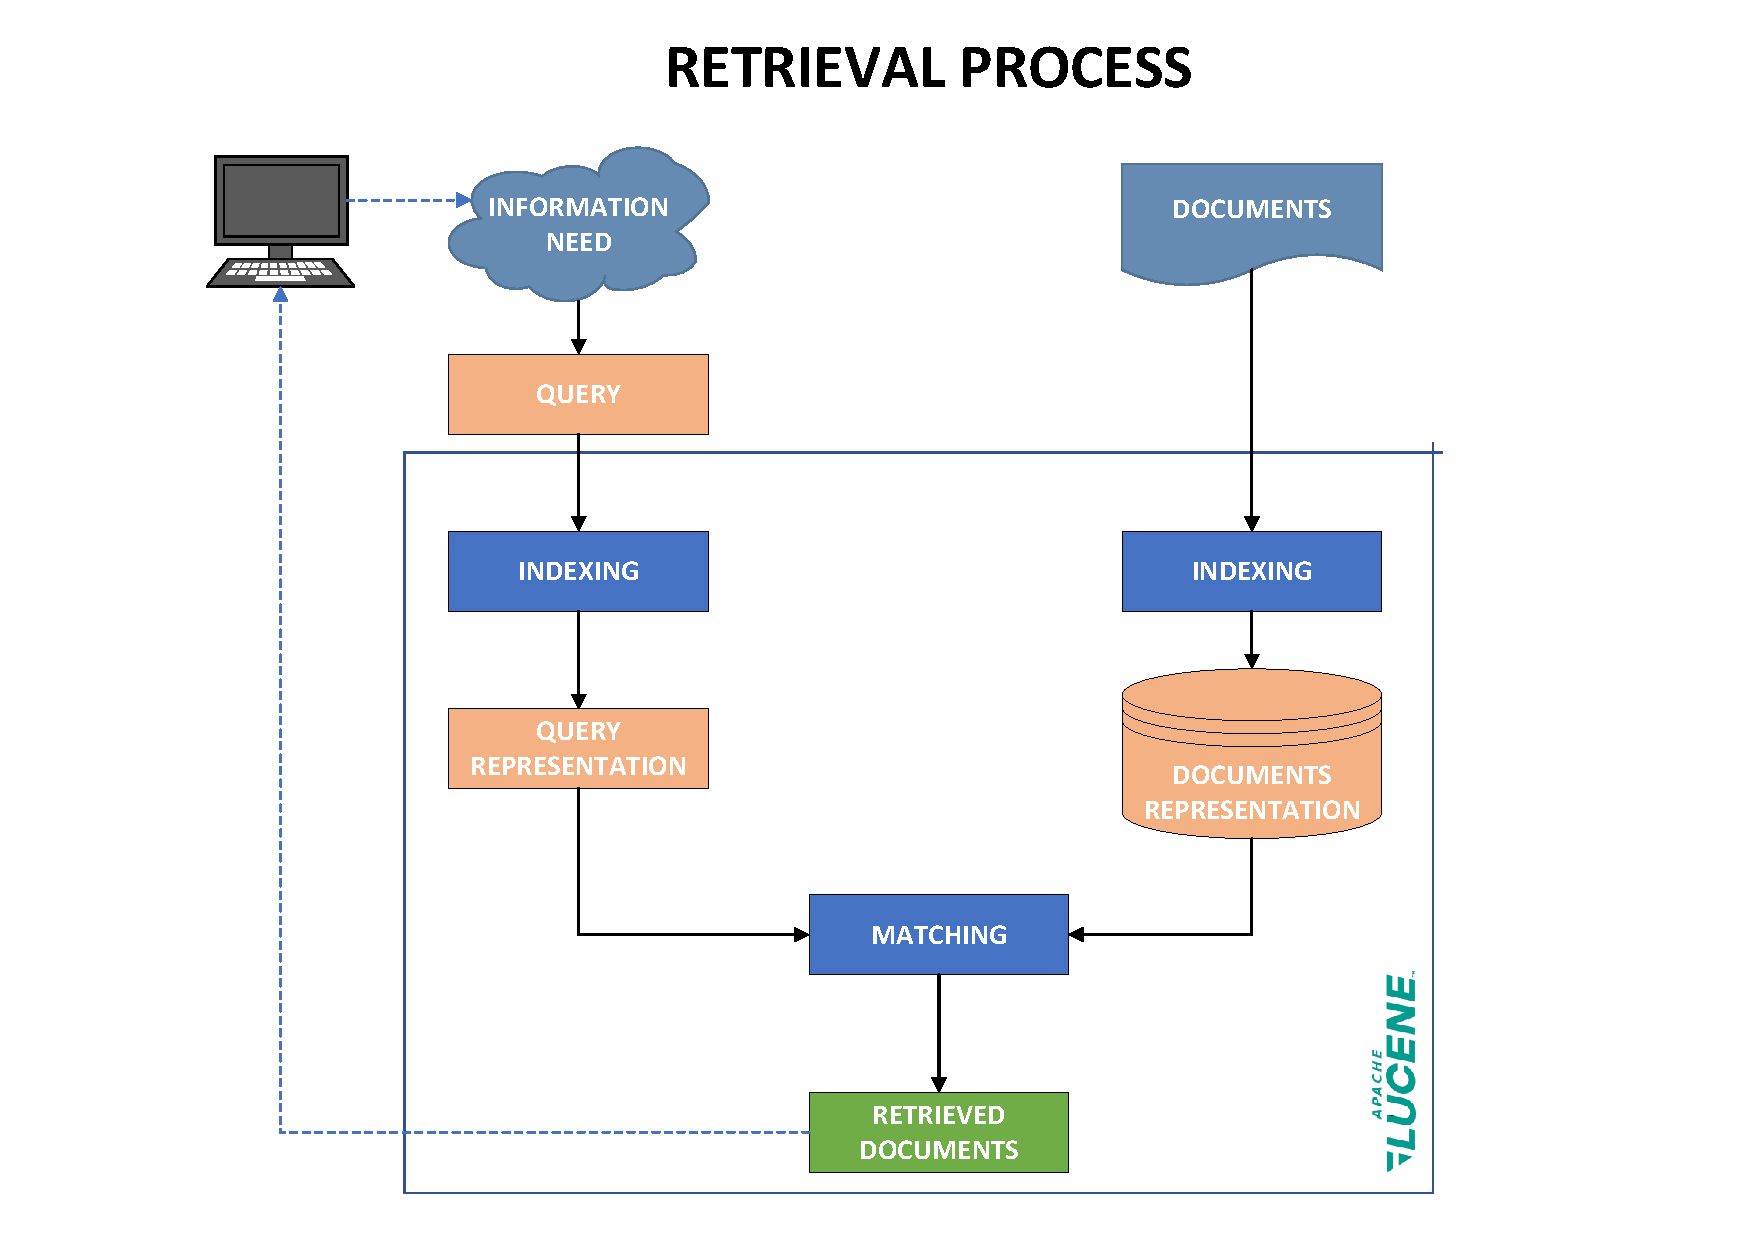
\includegraphics[width=0.9\linewidth]{figure/Y.pdf}
    \caption{Apache Lucene Y Model.}
    \label{fig:lucene_yModel}
\end{figure}

The workflow of our system, starting from the train collection provided by \ac{CLEF} \cite{cleflongeval}, is as follows:
\begin{enumerate}
    \item \textbf{Parsing}: The first phase consists of parsing the documents in the collection, which is a pre-processing operation performed to clean them from unnecessary noises. Since the collection is composed of web pages, the documents contain many leftovers like JavaScript scripts, HTML and CSS codes, HTTP and HTTPS URIs, and so on. The purpose of this phase is to ease the processing performed in the following phases.

    \item \textbf{Indexing}: Each parsed document is then analyzed and indexed keeping only the necessary information. Indexed documents are composed of two fields: an \textit{id} field, containing the identifier of the document in the collection, and a \textit{content} field, containing the entire body of the document cleaned by the parsing and indexing phases.

    \item \textbf{Query Formulation}: Topics are then parsed using the same analyzer used for documents, and used to formulate queries. For each topic, together with the already provided query, around 15 others are computed and used altogether for searching relevant documents.

    \item \textbf{Re-ranking}: The retrieved documents are re-ranked combining the scores obtained with two different approaches which compute the similarity of the document to the query given in the topic.

\end{enumerate}

\begin{figure}[!h]
    \centering
    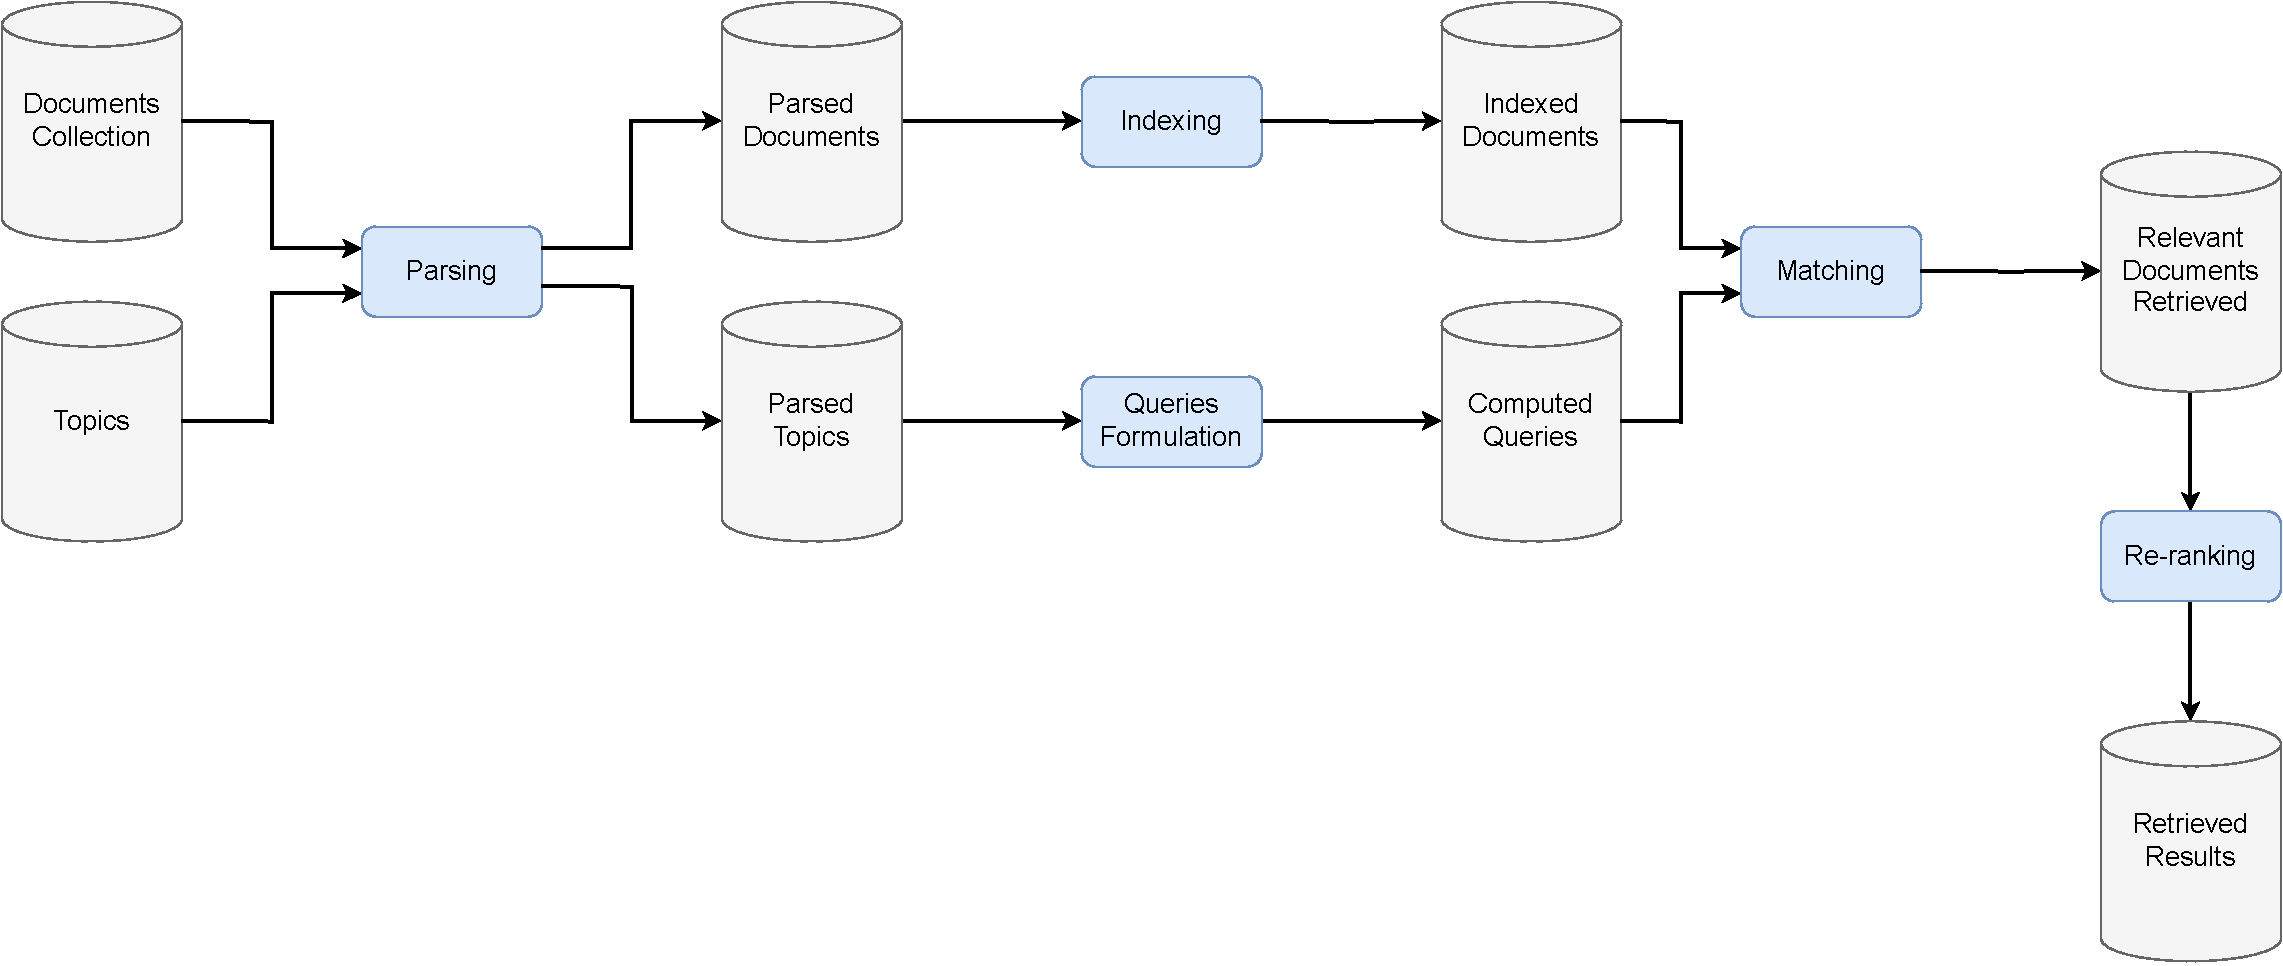
\includegraphics[width=\textwidth, height=\textheight, keepaspectratio]{figure/CLOSE_IR_Workflow (2).pdf}
    \caption{Workflow of the IR system implemented by \textit{CLOSE}.}
    \label{fig:CLOSE_IR_Workflow}
\end{figure}

\subsection{Project Structure}
The project is developed mainly in \textit{Java}, with the addition of some \textit{Python} scripts for performing the expansion of the queries and for the re-ranking of the retrieved documents for each topic. The overall structure is as follows:
\begin{itemize}
    \item \textbf{experiment}: This folder contains the results of the indexing obtained with different approaches, stored in different sub-folders.

    \item \textbf{python\_scripts}: This folder contains the above-mentioned \textit{Python} scripts, together with other \textit{txt} and \textit{JSON} data files produced or read by these scripts (i.e. query expansions, synonyms, etc.).

    \item \textbf{src/main/java}: This folder contains all the \textit{Java} classes used for the implementation of the \ac{IR} system, divided into the following packages:
    \begin{itemize}
        \item \textbf{parser}: This package contains the classes involved in the pre-processing of the document, i.e., the parsing phase.

        \item \textbf{analyzer}: This package contains the classes used for analyzing the parsed documents and topics of the collection.

        \item \textbf{indexer}: This package performs the indexing of the documents processed by the analyzer.

        \item \textbf{searcher}: Once the documents are indexed, the queries contained in the topics of the collection are parsed and then expanded in this package. Relevant (or assumed to be so) documents are retrieved and scored.

        \item \textbf{utils}: This package contains general utility classes, one of which performs the re-ranking of the documents retrieved by the \textit{searcher}.
    \end{itemize}
\end{itemize}

\vspace{\baselineskip}
A schema of the overall project structure is the following:
\begin{lstlisting}
    /code
    |------ experiment
    |------ python_scripts
    |------ src
               |------ main
                          |------ java
                                     |------ parser
                                     |------ analyzer
                                     |------ indexer
                                     |------ searcher
                                     |------ utils
\end{lstlisting}

\newpage
\begin{sidewaysfigure}[htp]
    \vspace*{\fill}
    
      \centering
      
      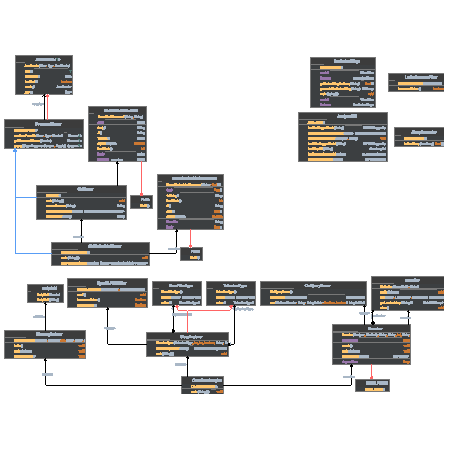
\includegraphics[ width=\linewidth]{figure/Classes_diagram_white_crop.pdf}
      
      \caption{Functional Decomposed Data Structure}
    
    \vfill
\end{sidewaysfigure}
\clearpage






\subsection{Parser} \label{parser_subsec}
As stated before, the documents in the collection provided by the \ac{CLEF} \textit{LongEval LAB 2023} \cite{cleflongeval} are essentially the corpus of web pages, to better represent the nature of a web test collection.
From this, the need for performing a pre-processing phase of parsing the documents before analyzing and indexing them arises.
In this phase, the documents are cleaned from all the residuals of codes not useful for our purposes. 
We first created an abstract class \textit{DocumentParser} and then extended it by implementing a custom \textit{ClefParser} class, which contains many functions for removing sundry types of noises that can be present in documents. 
This was the result of the trial and error approach we adopted for implementing this class:
\begin{itemize}
\item We started by reading a large statistical sample size of the documents in the collection to decide which types of noises needed to be removed.
\item Then we implemented the parser and ran it.
\item The results of the parsing were stored, and a sample of the parsed documents was analyzed to start this procedure again.
\end{itemize}

\begin{figure}[!h]
    \centering
    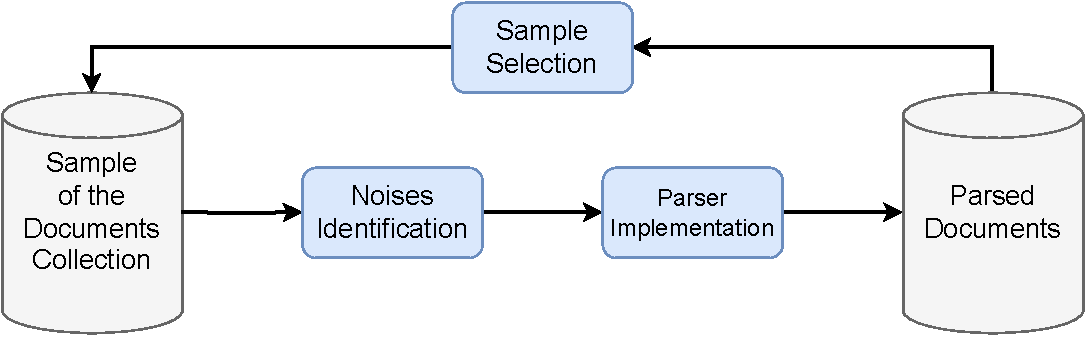
\includegraphics[width=0.8\linewidth]{figure/Parser_implementation_workflow.pdf}
    \caption{Workflow of the parser implementation.}
    \label{fig:Parser_implementation_workflow}
\end{figure}

The types of noises we tried to remove are the following:
\begin{itemize}
\item \textit{JavaScript} scripts,
\item \textit{HTTP} and \textit{HTTPS} URIs,
\item \textit{HTML} tags and \textit{CSS} stylesheets,
\item \textit{XML} and \textit{JSON} codes,
\item Meta tags and document properties,
\item Navigation menus,
\item Advertisements,
\item Footers,
\item Social media handlers,
\item Hashtags and mentions.
\end{itemize}

\newpage
We also identified some patterns of words and symbols to remove:
\begin{itemize}
\item Two words separated by an underscore, like \textit{word1\_word2}
\item Two words separated by a colon, like \textit{word1:word2}
\item Two words separated by a point, like ``\textit{word1.word2}''
\end{itemize}
We used \textit{Regular Expressions} \cite{regexdefinition} to define the patterns to identify and remove. 
The code below shows the \textit{removePatterns} function, used by the parser for removing the patterns mentioned above together with the \textit{HTTP} and \textit{HTTPS} URIs.
\begin{lstlisting}[language=Java]
    // Function to remove patterns like "word1_word2", "word1.word2", "word1.word2", and HTTP/HTTPS URIs from a string
    public String removePatterns(String input) {

        // Define regular expression pattern to match the desired patterns
        Pattern pattern = Pattern.compile("(\\w+)[_.:](\\w+) |
            (https?://[\\w-]+(\\.[\\w-]+)+([\\w.,@?^=%&:/~+#-]*[\\w@?^=%&/~+#-])?)
            ");
            
        // Replace all matched patterns with a space character
        Matcher matcher = pattern.matcher(input);
        String output = matcher.replaceAll(" ");

        return output;
    }
\end{lstlisting}

After different tries, we decided to use only the function above for removing noises, which gave an improving in \ac{MAP} of +0.5\%, together with another one used to remove \textit{JavaScript} codes, which by itself gave +3\% on \ac{MAP}. \\
The code of the \textit{JavaScript} parser function is the one below:
\begin{lstlisting}[language=Java]
    public String removeJavaScript(String documentBody) {
        // Get the body of the document.
        StringBuilder bodyBuilder = new StringBuilder(documentBody);

        //compiles regular expression for JS and all caps text
        Pattern jspattern=Pattern.compile("function.(.)[{]");

        int start=0;
        int end=0;
        //removes all <scripts>
        while((start=bodyBuilder.indexOf("<script", start))!=-1){
            if((end=bodyBuilder.indexOf("script>", start))!=-1){
                end=end+7;
                bodyBuilder.replace(start, end, "");
                continue;
            }
            if((end=bodyBuilder.indexOf(">", start))!=-1){
                end++;
                bodyBuilder.replace(start, end, "");
                continue;
            }
            start++;
        }

        //removes JS
        Matcher m = jspattern.matcher(bodyBuilder);
        while(m.find()){
            start=m.start();
            int count=1;
            for(int i=start; i<bodyBuilder.length(); i++){
                if(bodyBuilder.charAt(i)=='{'){
                    count++;
                    continue;
                }
                if((bodyBuilder.charAt(i)=='}')){
                    if(--count==0){
                        bodyBuilder.replace(start, i, "");
                        m = jspattern.matcher(bodyBuilder);
                        break;

                    }
                }
            }
        }

        return bodyBuilder.toString();
    }
\end{lstlisting}

The structure of the parsed document is defined in the \textit{ParsedTextDocument} class, and it is composed of just two fields, as provided by \ac{CLEF}:
\begin{enumerate}
\item \textit{id}: the identifier of the document,
\item \textit{body}: the (parsed) content of the document.
\end{enumerate}
The constructor of \textit{ParsedTextDocument} is the following:
\begin{lstlisting}[language=Java]
    /**
     * Creates a new parsed document.
     *
     * @param id  the document identifier.
     * @param body the document body.
     */
    public ParsedTextDocument(final String id, final String body) 
\end{lstlisting}
Inside it, multiple controls about the validity and integrity of the parameters are performed, then an object of the class is instantiated. \\
The class also contains the following utility methods:
\begin{itemize}
\item \textit{getIdentifier}, which returns the (unique) document identifier,
\item \textit{getBody}, which returns the body of the document,
\item \textit{toString}, which returns a \textit{String} representation of the document,
\item \textit{hashCode}, which returns the hash code of the document identifier,
\item \textit{equals(Object o)}, which returns true if the two objects have the same identifier.
\end{itemize}


\subsection{Analyzer} \label{analyzer_subsec}
The Analyzer is responsible for analyzing the extracted documents and preparing them for the Indexing and Searching phases. 
It does so by combining a series of techniques of text processing such as tokenization, stemming, stopword removal, and many more.\\
We extended Apache Lucene's Analyzer abstract class \cite{luceneanalyzer} by creating a custom class \textit{CloseAnalyzer}, which is fully customizable by its parameters that can be chosen when creating an instance of the class. 
This has been done because we tried different settings and approaches to maximize the results and kept all the possible variations as optional settings.
This \textit{CloseAnalyzer} is passed as a parameter and then used by the \textit{DirectoryIndexer} and by the \textit{Searcher}. \\
The constructor of \textit{CloseAnalyzer} accepts the following parameters:
\begin{itemize}
  \item \textbf{tokenizerType}: used to choose between three standard \textit{Lucene} tokenizers: \textit{WhitespaceTokenizer} \cite{lucenetokenizer}, \textit{LetterTokenizer} \cite{lucenelettertokenizer}, and \textit{StandardTokenizer} \cite{lucenestandardtokenizer}.
  
  \item \textbf{stemFilterType}: the possible choices for the stemming types are four standard \textit{Apache Solr} \cite{solr} filters: \textit{EnglishMinimalStemFilter} \cite{solrminimalstemfilter}, \textit{KStemFilter} \cite{solrkstemfilter}, \textit{PorterStemFilter} \cite{solrporterstemfilter}, and \textit{FrenchLightStemFilter} \cite{solrfrenchlightstemfilter}. 
  We also tried using \textit{FrenchMinimalStemFilter} \cite{solrfrenchminimalstemfilter} and a custom filter called \textit{LovinsStemmerFilter} based off a LovinsStemmer \cite{lucenelovinsstemmer} implementation but decided to keep them commented as they didn't improve the results.
  
  \item \textbf{minLength} and \textbf{maxLength}: these are integers that simply specify the minimum and maximum length of a token, applying Lucene's \textit{LengthFilter} \cite{lucenelengthfilter}.
  
  \item \textbf{isEnglishPossessiveFilter}: specifies whether to use Lucene's \textit{EnglishPossessiveFilter} \cite{luceneenglishpossessivefilter} or not. 
  Of course, this can be useful when operating with the English dataset.
  
  \item \textbf{stopFilterListName}: with this parameter, it's possible to insert the path of an eventual word stoplist \textit{.txt} file located in the \textit{resources} folder. 
  To do this we use Lucene's \textit{StopFilter} \cite{lucenestopfilter} and a custom class called \textit{AnalyzerUtil} that uses a \textit{loadStopList} method to read and load all the stoplist words from the specified file. 
  The stoplists we created are based on the standard ones but modified after inspecting the index with the \textit{Luke} \cite{luke} tool. 
  We have lists of different lengths and different ones for French and English.
  
  \item \textbf{nGramFilterSize}: if specified, this parameter is used to define the size of the n-grams to be applied by Lucene's \textit{NGramTokenFilter} \cite{lucenengramtokenfilter}.
  
  \item \textbf{shingleFilterSize}: similar to the previous one, if used, this integer number indicates the shingle size to be applied by Lucene's \textit{ShingleFilter} \cite{luceneshinglefilter} that allows the creation of a combination of words.
  
  \item \textbf{useNLPFilter}: this boolean allows the use of Solr's \cite{solr} \textit{OpenNLPPPOSFilter} \cite{solropennlpposfilter} for Part-Of-Speech Tagging and of a custom class called \textit{OpenNLPNERFilter} for Named Entity Recognition. 
  To load the \textit{.bin} models, which are located in the \textit{resources} folder, we use two methods from \textit{AnalyzerUtil}: \textit{loadPosTaggerModel} and \textit{loadNerTaggerModel}.
  
  \item \textbf{lemmatization}: specifies whether to use Solr's \textit{OpenNLPLemmatizerFilter} \cite{solropennlplemmafilter} by loading a \textit{.bin} model file in the \textit{resources} folder using AnalyzerUtil's \textit{loadLemmatizerModel} function.
  
  \item \textbf{frenchElisionFilter}: we applied this only when using the French dataset by adding Lucene's \textit{ElisionFilter} \cite{luceneelisionfilter} with an array of the following characters: 'l', 'd', 's', 't', 'n', 'm'.
\end{itemize}
On top of this, a \textit{LowerCaseFilter} \cite{lucenelowercasefilter} is always applied. \\
We also tried Lucene's \textit{ASCIIFoldingFilter} \cite{luceneasciifoldingfilter} and \textit{SynonymGraphFilter} \cite{lucenesynonymgraphfilter}. 
For the second one, only for the French Dataset, we used a \textit{SynonymMap} \cite{lucenesynonymmap} based on a \textit{.txt} file containing French synonyms.
\newline
After different trials with different variations of the parameter, the following is the instance of the \textit{CloseAnalyzer} we used:

\begin{lstlisting}
final Analyzer closeAnalyzer = new CloseAnalyzer(CloseAnalyzer.TokenizerType.Standard, 2, 15, false, "new-long-stoplist-fr.txt", CloseAnalyzer.StemFilterType.French, null, null, false, false, true);
\end{lstlisting}
We have opted for the French dataset and by doing so we have the \textit{StandardTokenizer}, 2 and 15 as minimum and maximum token length, we use \textit{frenchElisionFilter}, \textit{FrenchLightStemFilter}, and a list of 662 French words as a stoplist. 
We didn't use any of the other parameters.
We utilized the Gson library to efficiently parse a JSON files that contained query expansions. By leveraging Gson's capabilities, we were able to seamlessly convert the JSON data into Java objects, enabling effortless manipulation and integration of the query expansions into our application.


\subsection{Indexer}
The \textit{Indexer} is in charge of calling the \textit{Parser} (\ref{parser_subsec}) and the \textit{Analyzer} (\ref{analyzer_subsec}), taking the document processed by these two and indexing them as an object of the \textit{ParsedTextDocument} defined in the \textit{Parser}. \\
The class which performs the document processing mentioned above is \textit{DirectoryIndexer}, whose constructor is the following:
\begin{lstlisting}
    public DirectoryIndexer(final Analyzer analyzer, final Similarity similarity, final int ramBufferSizeMB,
                            final String indexPath, final String docsPath, final String extension,
                            final String charsetName, final long expectedDocs,
                            final Class<? extends DocumentParser> dpCls) {
\end{lstlisting}
It takes the following inputs:
\begin{itemize}
\item \textbf{analyzer}: the \textit{Analyzer} to be used, in our case \textit{CloseAnalyzer};
\item \textbf{similarity}: the \textit{Similarity} function to be used by the \textit{Analyzer};
\item \textbf{ramBufferSizeMB}: the size in megabytes of the RAM buffer for indexing the documents;
\item \textbf{indexPath}: the directory where to store the index;
\item \textbf{docsPath}: the directory from which the documents of the collection have to be read;
\item \textbf{extension}: the extension of the files in the collection to be indexed;
\item \textbf{charsetName}: the name of the charset used for encoding documents;
\item \textbf{expectedDocs}: the total number of documents expected to be indexed;
\item \textbf{dpCls}: the class of the \textit{DocumentParser} to be used, in our case \textit{ClefParser}.
\end{itemize}
The function which actually performs the storing of the index is:
\begin{verbatim}
public void index()
\end{verbatim}
Its main functionality, which consists of reading, indexing, and storing the processed documents, is shown below:
\begin{lstlisting}
    // Create a stream of parsed documents from the file with the given Parser class(dpCls)
    DocumentParser.create(dpCls, Files.newBufferedReader(file, cs)).forEach(pd -> {
        Document doc = new Document();
        ParsedTextDocument ptd = (ParsedTextDocument) pd;

        // add the document identifier
        doc.add(new StringField(ParsedTextDocument.Fields.ID, ptd.getIdentifier(), Field.Store.YES));

        // add the processed document content
        doc.add(new BodyField(ptd.getBody()));
        try {
            writer.addDocument(doc);
        } catch (IOException e) {
            e.printStackTrace();
        }

        docsCount++;

        // print progress every 10000 indexed documents
        if (docsCount % 10000 == 0) {
            System.out.printf("%d document(s) (%d files, %d Mbytes) indexed in %d seconds.%n",
            docsCount, filesCount, bytesCount / MBYTE,
            (System.currentTimeMillis() - start) / 1000);
        }
    });
\end{lstlisting}

The \textit{Indexer} contains some printouts used to see the progress of the indexing during the execution, such as the number of indexed documents, the time elapsed, if the number of documents indexed is less than expected, and some other eventual warning that can come out during this operation. \\
The overall workflow, starting from the documents collection and ending with having the indexed documents stored, is the following:
\begin{figure}[!h]
    \centering
    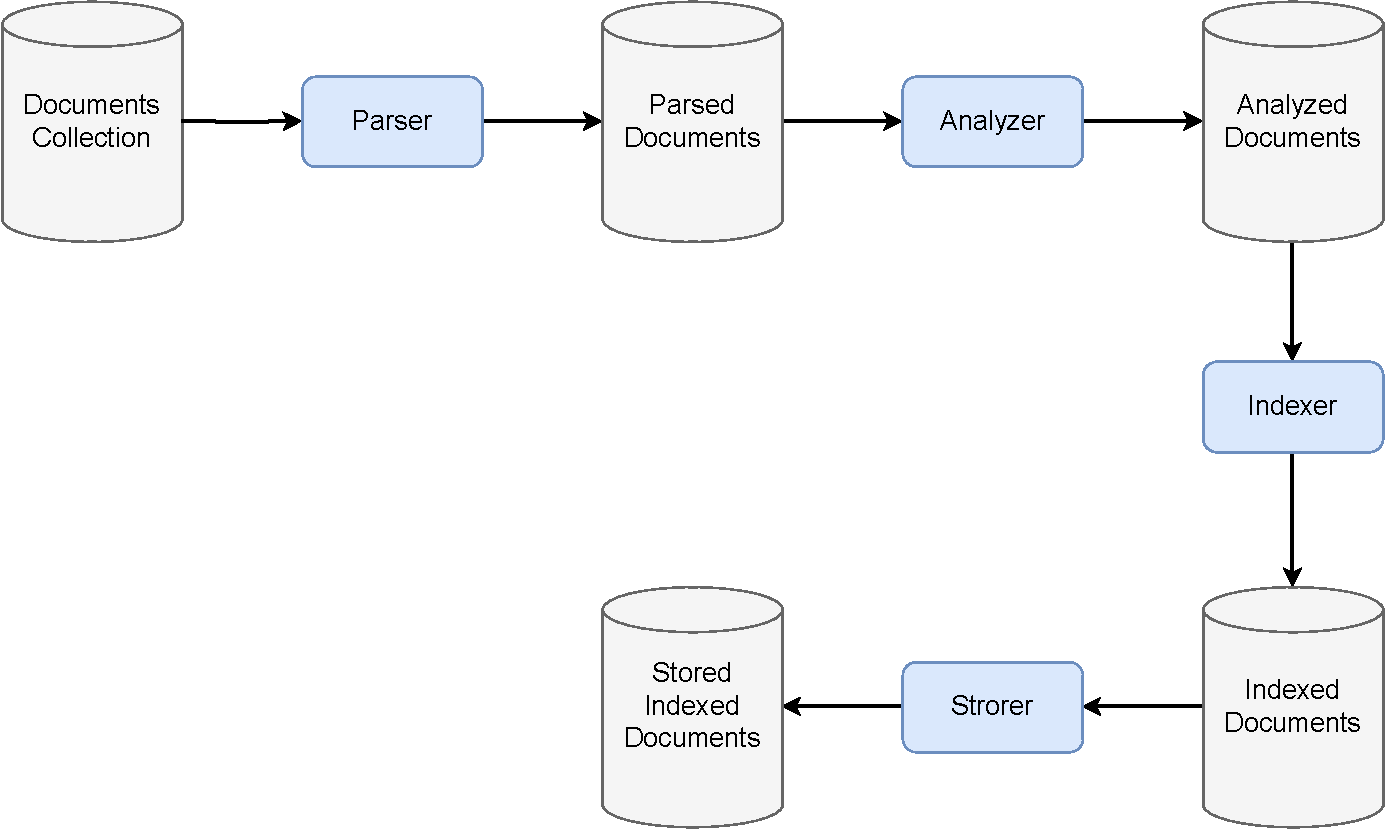
\includegraphics[width=0.8\linewidth]{figure/Indexer_workflow.pdf}
    \caption{Workflow of the indexer.}
    \label{fig:Indexer_workflow}
\end{figure}


\subsection{Searcher} \label{searcher_subsec}
The purpose of the \textit{Searcher} is to search through the indexed documents to retrieve relevant information based on user queries after analyzing them and to
return a ranked list of documents that match the user’s information needs.
\newline
Our implementation does so by accepting the following parameters:
\begin{itemize}
  \item \textbf{analyzer}: in this case, an instance of \textit{CloseAnalyzer}.
  \item \textbf{similarity}: we decided to opt for the \textit{BM25Similarity} \cite{lucenebm25similarity} function with the parameters \textit{k1} and \textit{b} tuned at 1.2 and 0.90.
  \item \textbf{Run options}: there are parameters for the index path, the topics path, the run path and the run name, the number of the expected topic (in our case 50), and the maximum number of documents retrieved (in our case 1000).
  \item \textbf{useEmbeddings}: a boolean value to decide whether to use embeddings or not. 
  If it is set to true we don't use the similarity function. In our implementation, we opted to not use them.
  \item \textbf{reRankModel}: this is the type of model used to do a Re-Ranking on the retrieved documents. 
  In our case, we use a model called \textit{all-MiniLM-L6-v2} \cite{huggingfaceallminilml6v2}, explained in the following subsection. 
  If the parameter is set to null, no model is used and the documents are scored normally.
\end{itemize}


\subsubsection{Query Expansion}
When running the search function, one of the first actions performed is to generate new queries from the original ones by query expansion.
We created a Python script that, given the \textit{*.trec} file, generates all the expanded terms for each query and stores everything in a \textit{.json} file called \textit{result}.
\newline
We use \textit{OpenAI's} \textit{Text completion} \cite{openaicompletionapi} endpoints to generate the expansions, we can use our need as prompt and the model will generate the result. 
We used the \textit{davinci} model, which is the most powerful one, and we set the \textit{temperature} parameter to 0.6, which is the value that gives the best results.
\newline
The sample result for prompt 
\begin{center}
    \textit{``Expand the following query with {num\_expansions} related terms or phrases for information retrieval (search-engine): {query} and the result should be in array format without any numbers at first [expanded\_term1, expanded\_term2, ...]''}     
\end{center}
is:
\begin{table}[H]
    \begin{tabular}{|l|l|l|}
        \hline
        Query                 & text-davinci-002                                                                                                                                                                  & text-davinci-003                                                                                                                                                                    \\ \hline
        antivirus comparaison & \begin{tabular}[c]{@{}l@{}}1. Antivirus software\\ 2. Antivirus protection\\ 3. Best antivirus\\ 4. Free antivirus\\ 5. Antivirus for Windows\\ 6. Antivirus for Mac\end{tabular} & \begin{tabular}[c]{@{}l@{}}1. Antivirus Reviews \\ 2. Antivirus Software \\ 3. Antivirus Protection \\ 4. Malware Protection \\ 5. Virus Scanner \\ 6. Online Security\end{tabular} \\ \hline
    \end{tabular}
    \label{tab:query_expansion}
\end{table}
The main difference between \textit{davinci-text-002} and \textit{davinci-text-003} is that the latter has been trained on a larger dataset, allowing it to generate more accurate results \cite{davincicomparison}.


\enlargethispage{2\baselineskip}
\subsubsection{Query Boosting}
Query boosting is a technique used to assign greater relevance to certain query terms or queries.\newline
We tried the following approach that seemed to improve the overall results: when building the queries in the search function of the \textit{Searcher} (\ref{searcher_subsec}), for each query, a \textit{BooleanQuery} \cite{lucenebooleanquery} is built in the following way: 
after getting the query expansions, each of them is added to the \textit{BooleanQuery} with the clause \textit{SHOULD} (meaning that at least one of them must be satisfied) and a main query is added with the clause \textit{MUST}, indicating that it must be satisfied. \\
This main query is boosted using Lucene's \textit{BoostQuery} \cite{luceneboostquery}, with a boost value tuned at 14.68 multiplied by the number of expansions.

\subsubsection{Document Re-Ranking}
This is the process of ranking the documents retrieved by the search function of the \textit{Searcher} (\ref{searcher_subsec}) a second time, using, in our case, a model that maps sentences and paragraphs to a 384-dimensional dense vector space called \textit{all-MiniLM-L6-v2}~\cite{huggingfaceallminilml6v2}. This sentence transformer model is coming from a Python framework called \textit{Sentence Transformers}~\cite{sentence-transformers}, also \textit{all-MiniLM-L6-v2} aims to train sentence embedding models on very large sentence level datasets using a self-supervised contrastive learning objective.
\newline
It works in the following way: in the constructor of the \textit{Searcher} the Re-Ranker is initialized and a predictor is created to perform inference.
At the end of the search function, we call a \textit{sort} function that, using the predictor, creates embeddings for the documents and, for each query, calculates the similarity between the query and the documents.
Finally, these scores are multiplied by the actual document's scores, and the documents are then sorted by looking at these new scores.
\newline
We tested different combinations of parameters to find the best one, and we found that the best combination is multiplying the document's score by the \textit{BM25Similarity} function, with the similarity calculated with the \textit{cosine} function.
\begin{figure}[!ht]
    \centering
    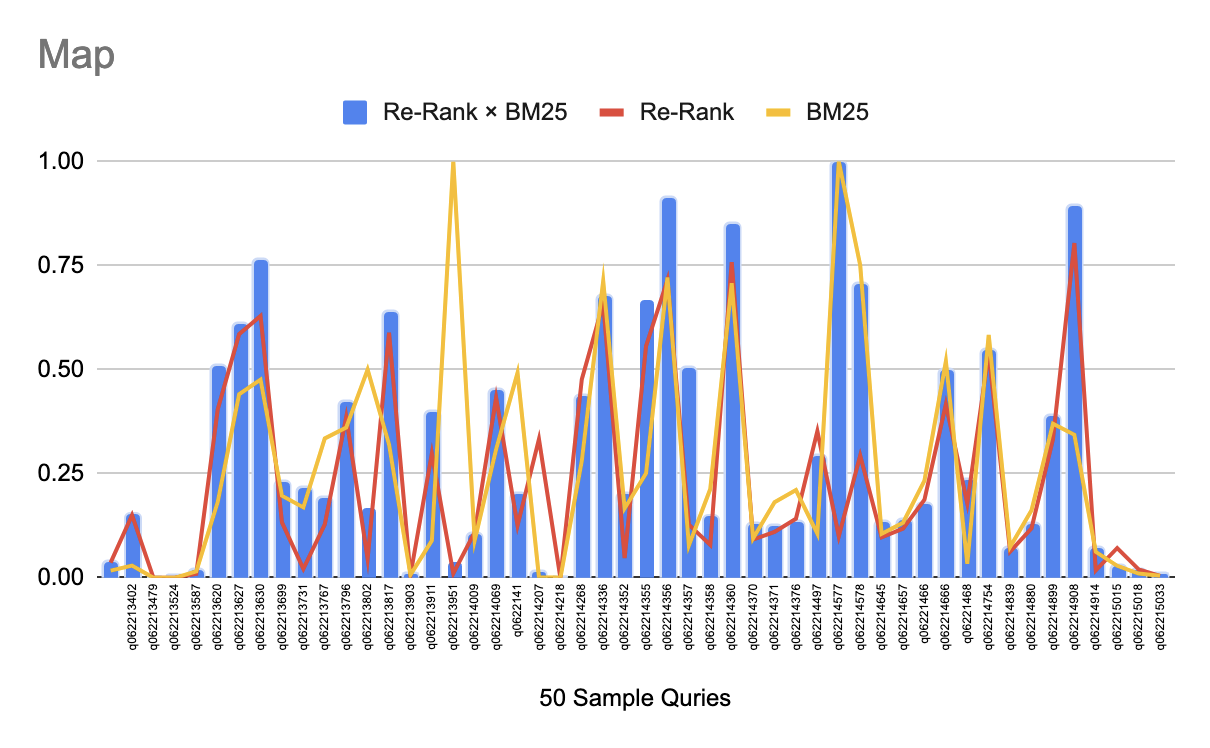
\includegraphics[scale=0.45, keepaspectratio]{figure/re-ranking}
    \caption{Plot of the re-ranking operation performed on 50 sample queries}
    \label{fig:re-rankinge}
\end{figure}
